\section{Preliminaries}
\subsection{Figure for the Main Theorem}
\label{sec:figmain}

\begin{figure*}[h]
\centering

\subfigure[$\textsc{PIS}(n, k, q)$ and $\textsc{PDS}(n, k, p, q)$ with $p = cq = \tilde{\Theta}(n^{-\alpha})$]{
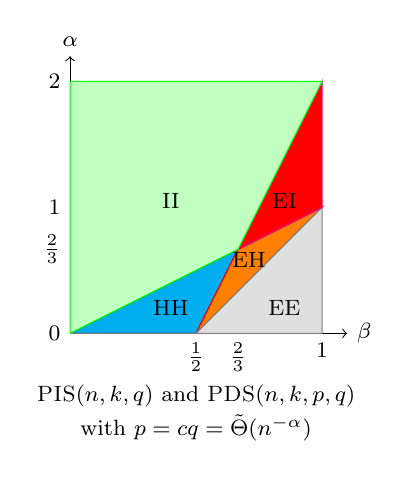
\begin{tikzpicture}[scale=0.32]
\tikzstyle{every node}=[font=\footnotesize]
\def\xmin{0}
\def\xmax{11}
\def\ymin{0}
\def\ymax{11}

\draw[->] (\xmin,\ymin) -- (\xmax,\ymin) node[right] {$\beta$};
\draw[->] (\xmin,\ymin) -- (\xmin,\ymax) node[above] {$\alpha$};

\node at (5, 0) [below] {$\frac{1}{2}$};
\node at (6.66, 0) [below] {$\frac{2}{3}$};
\node at (10, 0) [below] {$1$};
\node at (0, 0) [left] {$0$};
\node at (0, 10) [left] {$2$};
\node at (0, 3.33) [left] {$\frac{2}{3}$};
\node at (0, 5) [left] {$1$};

\filldraw[fill=cyan, draw=blue] (0,0) -- (5, 0) -- (6.66, 3.33) -- (0, 0);
\filldraw[fill=orange, draw=red] (5, 0) -- (6.66, 3.33) -- (10, 5) -- (5, 0);
\filldraw[fill=gray!25, draw=gray] (5, 0) -- (10, 5) -- (10, 0) -- (0, 0) -- (0, 0) -- (5, 0);
\filldraw[fill=red, draw=magenta] (6.66, 3.33) -- (10, 5) -- (10, 10) -- (6.66, 3.33);
\filldraw[fill=green!25, draw=green] (0, 0) -- (6.66, 3.33) -- (10, 10) -- (0, 10) -- (0, 0);

\node at (4, 1) {HH};
\node at (8.5, 1) {EE};
\node at (7.1, 2.9) {EH};
\node at (8.5, 5.25) {EI};
\node at (4, 5.25) {II};
\node at (5, -2.5) {$\textsc{PIS}(n, k, q)$ and $\textsc{PDS}(n, k, p, q)$};
\node at (5, -3.75) {with $p = cq = \tilde{\Theta}(n^{-\alpha})$};
\end{tikzpicture}}
\quad
\subfigure[$\textsc{PDS}(n, k, p, q)$ with $q = \tilde{\Theta}(n^{-\alpha})$ and $p - q = \tilde{\Theta}(n^{-5\alpha/4})$]{
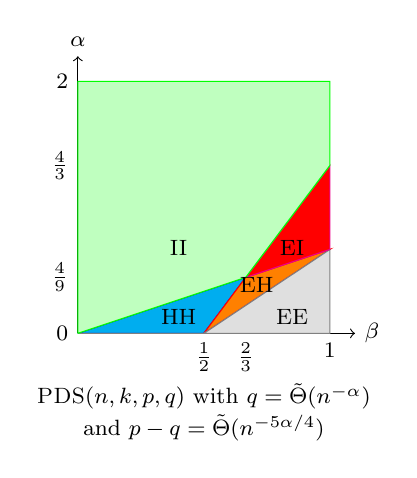
\begin{tikzpicture}[scale=0.32]
\tikzstyle{every node}=[font=\footnotesize]
\def\xmin{0}
\def\xmax{11}
\def\ymin{0}
\def\ymax{11}

\draw[->] (\xmin,\ymin) -- (\xmax,\ymin) node[right] {$\beta$};
\draw[->] (\xmin,\ymin) -- (\xmin,\ymax) node[above] {$\alpha$};

\node at (5, 0) [below] {$\frac{1}{2}$};
\node at (6.66, 0) [below] {$\frac{2}{3}$};
\node at (10, 0) [below] {$1$};
\node at (0, 0) [left] {$0$};
\node at (0, 10) [left] {$2$};
\node at (0, 2.22) [left] {$\frac{4}{9}$};
\node at (0, 6.66) [left] {$\frac{4}{3}$};

\filldraw[fill=cyan, draw=blue] (0,0) -- (5, 0) -- (6.66, 2.22) -- (0, 0);
\filldraw[fill=orange, draw=red] (5, 0) -- (6.66, 2.22) -- (10, 3.33) -- (5, 0);
\filldraw[fill=gray!25, draw=gray] (5, 0) -- (10, 3.33) -- (10, 0) -- (0, 0) -- (0, 0) -- (5, 0);
\filldraw[fill=red, draw=magenta] (6.66, 2.22) -- (10, 3.33) -- (10, 6.66) -- (6.66, 2.22);
\filldraw[fill=green!25, draw=green] (0, 0) -- (6.66, 2.22) -- (10, 6.66) -- (10, 10) -- (0, 10) -- (0, 0);

\node at (4, 0.66) {HH};
\node at (8.5, 0.66) {EE};
\node at (7.1, 1.92) {EH};
\node at (8.5, 3.4) {EI};
\node at (4, 3.4) {II};
\node at (5, -2.5) {$\textsc{PDS}(n, k, p, q)$ with $q = \tilde{\Theta}(n^{-\alpha})$};
\node at (5, -3.75) {and $p - q = \tilde{\Theta}(n^{-5\alpha/4})$};
\end{tikzpicture}}
\quad
\subfigure[$\textsc{SSBM}(n, k, q, \rho)$ with $q = \tilde{\Theta}(1)$ and $\rho = \tilde{\Theta}(n^{-\alpha})$]{
\centering
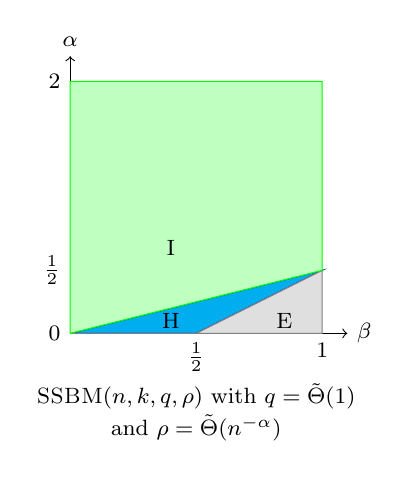
\begin{tikzpicture}[scale=0.32]
\tikzstyle{every node}=[font=\footnotesize]
\def\xmin{0}
\def\xmax{11}
\def\ymin{0}
\def\ymax{11}

\draw[->] (\xmin,\ymin) -- (\xmax,\ymin) node[right] {$\beta$};
\draw[->] (\xmin,\ymin) -- (\xmin,\ymax) node[above] {$\alpha$};

\node at (5, 0) [below] {$\frac{1}{2}$};
\node at (10, 0) [below] {$1$};
\node at (0, 0) [left] {$0$};
\node at (0, 10) [left] {$2$};
\node at (0, 2.5) [left] {$\frac{1}{2}$};

\filldraw[fill=cyan, draw=blue] (0,0) -- (5, 0) -- (10, 2.5) -- (0, 0);
\filldraw[fill=gray!25, draw=gray] (5, 0) -- (10, 2.5) -- (10, 0) -- (0, 0) -- (0, 0) -- (5, 0);
\filldraw[fill=green!25, draw=green] (0, 0) -- (10, 2.5) -- (10, 10) -- (0, 10) -- (0, 0);

\node at (4, 0.5) {H};
\node at (8.5, 0.5) {E};
\node at (4, 3.4) {I};
\node at (5, -2.5) {$\textsc{SSBM}(n, k, q, \rho)$ with $q = \tilde{\Theta}(1)$};
\node at (5, -3.75) {and $\rho = \tilde{\Theta}(n^{-\alpha})$};
\end{tikzpicture}}
\quad
\subfigure[$\textsc{BC}(n, k, \mu)$ with $\mu = \tilde{\Theta}(n^{-\alpha})$]{
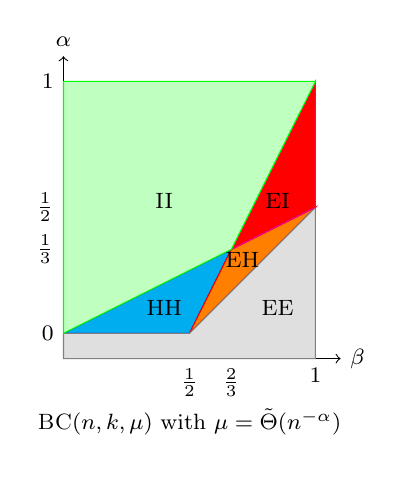
\begin{tikzpicture}[scale=0.32]
\tikzstyle{every node}=[font=\footnotesize]
\def\xmin{0}
\def\xmax{11}
\def\ymin{-1}
\def\ymax{11}

\draw[->] (\xmin,\ymin) -- (\xmax,\ymin) node[right] {$\beta$};
\draw[->] (\xmin,\ymin) -- (\xmin,\ymax) node[above] {$\alpha$};

\node at (5, -1) [below] {$\frac{1}{2}$};
\node at (6.66, -1) [below] {$\frac{2}{3}$};
\node at (10, -1) [below] {$1$};
\node at (0, 0) [left] {$0$};
\node at (0, 10) [left] {$1$};
\node at (0, 3.33) [left] {$\frac{1}{3}$};
\node at (0, 5) [left] {$\frac{1}{2}$};

\filldraw[fill=cyan, draw=blue] (0,0) -- (5, 0) -- (6.66, 3.33) -- (0, 0);
\filldraw[fill=orange, draw=red] (5, 0) -- (6.66, 3.33) -- (10, 5) -- (5, 0);
\filldraw[fill=gray!25, draw=gray] (5, 0) -- (10, 5) -- (10, -1) -- (0, -1) -- (0, 0) -- (5, 0);
\filldraw[fill=red, draw=magenta] (6.66, 3.33) -- (10, 5) -- (10, 10) -- (6.66, 3.33);
\filldraw[fill=green!25, draw=green] (0, 0) -- (6.66, 3.33) -- (10, 10) -- (0, 10) -- (0, 0);

\node at (4, 1) {HH};
\node at (8.5, 1) {EE};
\node at (7.1, 2.9) {EH};
\node at (8.5, 5.25) {EI};
\node at (4, 5.25) {II};
\node at (5, -3.5) {$\textsc{BC}(n, k, \mu)$ with $\mu = \tilde{\Theta}(n^{-\alpha})$};
\node at (5, -4.75) {};
\end{tikzpicture}}
\quad
\subfigure[$\textsc{ROS}(n, k, \mu)$ and $\textsc{SSW}(n, k, \mu)$ with $\frac{\mu}{k} = \tilde{\Theta}(n^{-\alpha})$]{
\centering
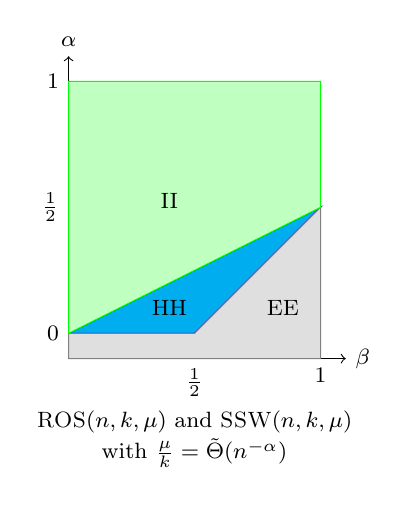
\begin{tikzpicture}[scale=0.32]
\tikzstyle{every node}=[font=\footnotesize]
\def\xmin{0}
\def\xmax{11}
\def\ymin{-1}
\def\ymax{11}

\draw[->] (\xmin,\ymin) -- (\xmax,\ymin) node[right] {$\beta$};
\draw[->] (\xmin,\ymin) -- (\xmin,\ymax) node[above] {$\alpha$};

\node at (5, -1) [below] {$\frac{1}{2}$};
\node at (10, -1) [below] {$1$};
\node at (0, 0) [left] {$0$};
\node at (0, 10) [left] {$1$};
\node at (0, 5) [left] {$\frac{1}{2}$};

\filldraw[fill=cyan, draw=blue] (0,0) -- (5, 0) -- (10, 5) -- (0, 0);
\filldraw[fill=gray!25, draw=gray] (5, 0) -- (10, 5) -- (10, -1) -- (0, -1) -- (0, 0) -- (5, 0);
\filldraw[fill=green!25, draw=green] (0, 0) -- (10, 5) -- (10, 10) -- (0, 10) -- (0, 0);

\node at (4, 1) {HH};
\node at (8.5, 1) {EE};
\node at (4, 5.25) {II};
\node at (5, -3.5) {$\textsc{ROS}(n, k, \mu)$ and $\textsc{SSW}(n, k, \mu)$};
\node at (5, -4.75) {with $\frac{\mu}{k} = \tilde{\Theta}(n^{-\alpha})$};
\end{tikzpicture}}

\subfigure[$\textsc{SPCA}(n, k, d, \theta)$ with $d = \Theta(n)$ and $\theta = \tilde{\Theta}(n^{-\alpha})$]{
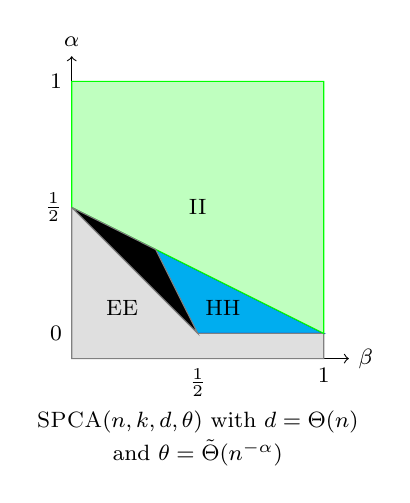
\begin{tikzpicture}[scale=0.32]
\tikzstyle{every node}=[font=\footnotesize]
\def\xmin{0}
\def\xmax{11}
\def\ymin{-1}
\def\ymax{11}

\draw[->] (\xmin,\ymin) -- (\xmax,\ymin) node[right] {$\beta$};
\draw[->] (\xmin,\ymin) -- (\xmin,\ymax) node[above] {$\alpha$};

\node at (5, -1) [below] {$\frac{1}{2}$};
\node at (10, -1) [below] {$1$};
\node at (0, 0) [left] {$0$};
\node at (0, 10) [left] {$1$};
\node at (0, 5) [left] {$\frac{1}{2}$};

\filldraw[fill=cyan, draw=blue] (0, 5) -- (10, 0) -- (5, 0) -- (0, 5);
\filldraw[fill=gray!25, draw=gray] (0, 5) -- (5, 0) -- (10, 0) -- (10, -1) -- (0, -1) -- (0, 5);
\filldraw[fill=green!25, draw=green] (0, 5) -- (10, 0) -- (10, 10) -- (0, 10) -- (0, 5);
\filldraw[fill=black, draw=gray] (0, 5) -- (3.33, 3.33) -- (5, 0) -- (0, 5);
\node at (6, 1) {HH};
\node at (2, 1) {EE};
\node at (5, 5) {II};
\node at (5, -3.5) {$\textsc{SPCA}(n, k, d, \theta)$ with $d = \Theta(n)$};
\node at (5, -4.75) {and $\theta = \tilde{\Theta}(n^{-\alpha})$};
\end{tikzpicture}}
\quad
\subfigure[$\textsc{BSPCA}(n, k, d, \theta)$ with $d = \Theta(n)$ and $\theta = \tilde{\Theta}(n^{-\alpha})$]{
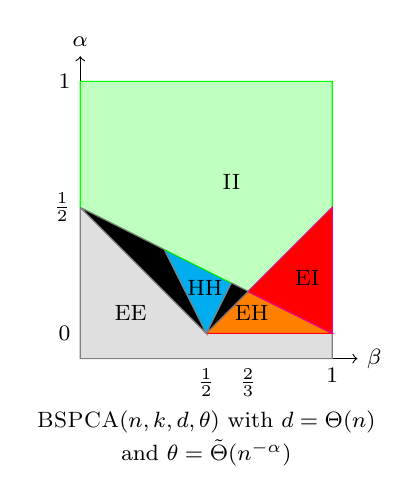
\begin{tikzpicture}[scale=0.32]
\tikzstyle{every node}=[font=\footnotesize]
\def\xmin{0}
\def\xmax{11}
\def\ymin{-1}
\def\ymax{11}

\draw[->] (\xmin,\ymin) -- (\xmax,\ymin) node[right] {$\beta$};
\draw[->] (\xmin,\ymin) -- (\xmin,\ymax) node[above] {$\alpha$};

\node at (5, -1) [below] {$\frac{1}{2}$};
\node at (6.66, -1) [below] {$\frac{2}{3}$};
\node at (10, -1) [below] {$1$};
\node at (0, 0) [left] {$0$};
\node at (0, 10) [left] {$1$};
\node at (0, 5) [left] {$\frac{1}{2}$};

\filldraw[fill=cyan, draw=blue] (0, 5) -- (6.66, 1.66) -- (5, 0) -- (0, 5);
\filldraw[fill=gray!25, draw=gray] (0, 5) -- (5, 0) -- (10, 0) -- (10, -1) -- (0, -1) -- (0, 5);
\filldraw[fill=green!25, draw=green] (0, 5) -- (6.66, 1.66) -- (10, 5) -- (10, 10) -- (0, 10) -- (0, 5);
\filldraw[fill=orange, draw=red] (5, 0) -- (6.66, 1.66) -- (10, 0) -- (5, 0);
\filldraw[fill=red, draw=magenta] (6.66, 1.66) -- (10, 5) -- (10, 0) -- (6.66, 1.66);
\filldraw[fill=black, draw=gray] (0, 5) -- (3.33, 3.33) -- (5, 0) -- (0, 5);
\filldraw[fill=black, draw=gray] (5, 0) -- (6, 2) -- (6.67, 1.67) -- (5, 0);

\node at (2, 0.8) {EE};
\node at (6, 6) {II};
\node at (4.95, 1.8) {HH};
\node at (6.8, 0.8) {EH};
\node at (9, 2.2) {EI};
\node at (5, -3.5) {$\textsc{BSPCA}(n, k, d, \theta)$ with $d = \Theta(n)$};
\node at (5, -4.75) {and $\theta = \tilde{\Theta}(n^{-\alpha})$};
\end{tikzpicture}}
\caption{Parameter regimes by problem plotted as signal vs. sparsity. Sparsity is $k = \tilde{\Theta}(n^{\beta})$. First labels characterize detection and second labels characterize exact recovery. Recovery is not considered for $\textsc{SSBM}$ and weak recovery is considered for $\textsc{SPCA}$ and $\textsc{BSPCA}$. In Easy (E) regimes, there is a polynomial-time algorithm. In Hard (H) regimes, the PC or PDS conjecture implies there is no polynomial-time algorithm. In Impossible (I) regimes, the task is information-theoretically impossible. Hardness in black regions is open.}
\label{fig:diagrams}
\end{figure*}

\pagebreak

\subsection{Hardness Results from an Algorithmic Perspective}

\begin{figure*}[t!]
\centering
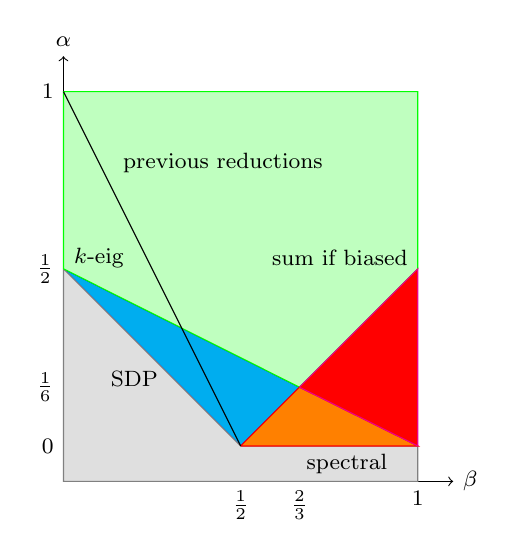
\begin{tikzpicture}[scale=0.45]
\tikzstyle{every node}=[font=\footnotesize]
\def\xmin{0}
\def\xmax{11}
\def\ymin{-1}
\def\ymax{11}

\draw[->] (\xmin,\ymin) -- (\xmax,\ymin) node[right] {$\beta$};
\draw[->] (\xmin,\ymin) -- (\xmin,\ymax) node[above] {$\alpha$};

\node at (5, -1) [below] {$\frac{1}{2}$};
\node at (6.66, -1) [below] {$\frac{2}{3}$};
\node at (10, -1) [below] {$1$};
\node at (0, 0) [left] {$0$};
\node at (0, 10) [left] {$1$};
\node at (0, 5) [left] {$\frac{1}{2}$};
\node at (0, 1.67) [left] {$\frac{1}{6}$};

\filldraw[fill=cyan, draw=blue] (0, 5) -- (6.66, 1.66) -- (5, 0) -- (0, 5);
\filldraw[fill=gray!25, draw=gray] (0, 5) -- (5, 0) -- (10, 0) -- (10, -1) -- (0, -1) -- (0, 5);
\filldraw[fill=green!25, draw=green] (0, 5) -- (6.66, 1.66) -- (10, 5) -- (10, 10) -- (0, 10) -- (0, 5);
\filldraw[fill=orange, draw=red] (5, 0) -- (6.66, 1.66) -- (10, 0) -- (5, 0);
\filldraw[fill=red, draw=magenta] (6.66, 1.66) -- (10, 5) -- (10, 0) -- (6.66, 1.66);
\draw (5, 0) -- (0, 10);

\node at (2, 1.9) {SDP};
\node at (1, 5.3) {$k$-eig};
\node at (8, -0.5) {spectral};
\node at (7.8, 5.3) {sum if biased};
\node at (4.5, 8) {previous reductions};
\end{tikzpicture}
\caption{Algorithms for sparse PCA with $d = \Theta(n)$, $k = \tilde{\Theta}(n^\beta)$ and $\theta = \tilde{\Theta}(n^{-\alpha})$. Lines represent the strongest guarantees of each algorithm. The line marked as previous reductions shows the strongest previously known planted clique lower bounds for sparse PCA when $k \lesssim \sqrt{n}$. No planted clique lower bounds were known for $k \gg \sqrt{n}$.}
\label{fig:algsspca}
\end{figure*}

In this section, we motivate our computational lower bounds and techniques using algorithms for sparse PCA as an example. Consider the detection problem for sparse PCA where either $X_1, X_2, \dots, X_n$ are sampled i.i.d. from $N(0, I_d)$ or are sampled i.i.d. from $N(0, I_d + \theta vv^\top)$ for some latent $k$-sparse unit vector $v$ with nonzero entries equal to $\pm 1/\sqrt{k}$. The task is to detect which of the two distributions the samples originated from. For now assume that $d = \Theta(n)$. Now consider the following four algorithms:
\begin{enumerate}
\item \textbf{Semidefinite Programming:} Form the empirical covariance matrix $\hat{\Sigma} = \frac{1}{n} \sum_{i = 1}^n X_i X_i^\top$ and solve the convex program
\begin{align*}
\max_Z \quad &\text{Tr}\left(\hat{\Sigma} Z\right) \\
\text{s.t.} \quad &\text{Tr}(Z) = 1, |Z|_1 \le k, Z \succeq 0
\end{align*}
As shown in \cite{berthet2013complexity}, thresholding the resulting maximum solves the detection problem as long as $\theta = \tilde{\Omega}(\sqrt{k^2/n})$.
\item \textbf{Spectral Algorithm:} Threshold the maximum eigenvalue of $\hat{\Sigma}$. If the data are sampled from $N(0, I_d)$, then the largest eigenvalue is with high probability at most
$$\lambda_{\text{max}}(\hat{\Sigma}) \le \frac{d}{n} + \sqrt{\frac{d}{n}} + 1 + o(1)$$
by standard bounds on the singular values of random Gaussian matrices. Since $d = \Theta(n)$, this algorithm succeeds as long as $\theta = \Omega(1)$. This algorithm was considered in \cite{krauthgamer2015semidefinite}.
\item \textbf{Sum Test:} Sum the entries of $\hat{\Sigma}$ and threshold the absolute value of the sum. If $v$ has sum exactly zero, then this test will not succeed. However, if we assume that $\hat{\Sigma}$ has even 51\% of its nonzero entries of one sign, then this test succeeds if $\theta = \tilde{\Omega}(\sqrt{n}/k)$.
\item \textbf{$k$-Sparse Eigenvalue:} Compute and threshold the $k$-sparse unit vector $u$ that maximizes $u^\top \hat{\Sigma} u$. This can be found by finding the largest eigenvector of each $k \times k$ principal submatrix of $\hat{\Sigma}$. Note that this takes exponential time. It was shown in \cite{berthet2013complexity} that this succeeds as long as $\theta = \tilde{\Omega}(\sqrt{k/n})$.
\end{enumerate}
The boundaries at which these algorithms begin to succeed are shown in Figure \ref{fig:algsspca} for the regime $k = \tilde{\Theta}(n^\beta)$ and $\theta = \tilde{\Theta}(n^{-\alpha})$. The computational lower bound mapping to $\theta \approx k^2/n$ in \cite{berthet2013complexity} and \cite{gao2017sparse} is also drawn. As shown, the only point in the parameter diagram for which it matches an algorithmic upper bound is $\alpha = 0$ and $\beta = 1/2$, corresponding to when $\theta = \tilde{\Theta}(1)$ and $k = \tilde{\Theta}(\sqrt{n})$.

For sparse PCA with $d = \Theta(n)$, the SDP is optimal up to $k = \Theta(\sqrt{n})$, at which point the spectral algorithm has stronger guarantees. This algorithmic transition at $k = \Theta(\sqrt{n})$ is characteristic of all of the problems we consider. For the biased variant of sparse PCA where the sum test succeeds, the sum test always does strictly better than the spectral algorithm. Furthermore, the biased variant ceases to have a statistical computational gap around $k = \Theta(n^{2/3})$. While the sum test yields an improved algorithm for detection, unlike the other three algorithms considered above, it does not translate into an algorithm for recovering the support of the sparse component. Given a conjecture about recovery in planted dense subgraph, we show that the best recovery algorithm for biased sparse PCA can only match the guarantees of the spectral algorithm. Thus the biased variant induces a detection-recovery gap when $k \gg \sqrt{n}$. We show that the disappearance of a statistical computation gap at $k = \Theta(n^{2/3})$ and a detection-recovery gap when $k \gg \sqrt{n}$ are features of the problems we consider that admit a sum test. These are biased sparse PCA, planted independent set, planted dense subgraph and biclustering. Distributional lifting gives tight planted clique lower bounds for these problems.

In contrast, rank-1 submatrix, the subgraph stochastic block model and sparse PCA do not admit a sum test. Given the planted clique conjecture, rank-1 submatrix and sparse PCA have no detection-recovery gap and retain their statistical-computational gap for all sparsities $k$. Reflection cloning shows tight lower bounds for these problems in the regime $k \gg \sqrt{n}$, where spectral algorithms become optimal. It is surprising that the planted clique conjecture can tightly capture completely different sets of computational barriers for different problems, illustrating its power as an average-case hardness assumption. Although analogues of the sum test, spectral algorithms and semidefinite programs all have equivalent guarantees up to logarithmic factors for planted clique, reductions from planted clique show tight hardness in problems for which this is not true.

\subsection{Prior Work}

This work is part of a growing body of literature giving rigorous evidence for computational-statistical gaps in high-dimensional inference problems. We focus on average-case reductions to directly relate computational-statistical gaps in different problems, as opposed to giving worst-case evidence for hardness in statistical problems \cite{zhang2014lower, hardt2014computational, chan2016approximability}. A survey of prior results on computational-statistical gaps with a focus on predictions from statistical physics can be found in \cite{bandeira2018notes} and a general analysis of gaps for algorithms from several convex relaxation hierarchies can be found in \cite{chandrasekaran2013computational}.

\paragraph{Planted Clique and Independent Set.} Our computational lower bounds are based on average-case reductions to the problem of finding a planted clique of size $k$ in an Erd\H{o}s-R\'{e}nyi graph with $n$ vertices. The planted clique problem was introduced in \cite{alon1998finding}, where a spectral algorithm was shown to recover the planted clique if $k = \Omega(\sqrt{n})$. A number of algorithms for planted clique have since been studied, including approximate message passing, semidefinite programming, nuclear norm minimization and several combinatorial approaches \cite{feige2000finding, mcsherry2001spectral, feige2010finding, ames2011nuclear, dekel2014finding, deshpande2015finding, chen2016statistical}. All of these algorithms require that $k = \Omega(\sqrt{n})$, which has led to the planted clique conjecture that no polynomial time algorithm can recover the planted clique if $k = o(\sqrt{n})$. It was also shown in \cite{alon2007testing}, recovering and detecting the planted clique are equivalent up to $\log n$ factors in $k$. There have been a number of previous average-case reductions from the planted clique conjecture, which we discuss in more detail in the prior work section on average-case reductions.

Several works have considered finding independent sets in sparse Erd\H{o}s-R\'{e}nyi graphs, similar to the regime with edge density $q = \tilde{\Theta}(n^{-\alpha})$ where $\alpha \in (0, 2)$ we consider here. In \cite{coja2015independent, gamarnik2014limits, rahman2017local}, the authors examine greedy and local algorithms to find independent sets in the regime $q = \tilde{\Theta}(n^{-1})$ in models related to Erd\H{o}s-R\'{e}nyi graphs. In \cite{feige2005finding}, a spectral algorithm is given to find a planted independent set in the regime $q = \tilde{\Theta}(n^{-1})$ and in \cite{coja2003finding}, the planted independent set recovery problem is shown to be possible in polynomial time in the regime $\alpha \in (0, 1)$ when $q \gg \frac{n}{k^2}$ even in a semirandom model. The algorithms of \cite{chen2016statistical} also apply to recovering planted independent sets after taking the complement of the input graph.

\paragraph{Planted Dense Subgraph and Community Detection.} The planted dense subgraph detection problem was considered in \cite{arias2014community, butucea2013detection, verzelen2015community, hajek2015computational} and generalizations of the recovery problem were considered in \cite{chen2016statistical, hajek2016information, montanari2015finding, candogan2018finding}. In \cite{hajek2015computational}, a reduction from planted clique was given for the regime $p = cq$ for some constant $c > 1$ and $q = \tilde{\Theta}(n^{-\alpha})$ and $k$ is binomially distributed, where $k$, $n$, $p$ and $q$ are the size of the community, size of the graph, community edge density and graph edge density, respectively. Our results strengthen this lower bound to apply for deterministic $k$ and for all $p > q$ with $p - q = O(q)$ where $q = \tilde{\Theta}(n^{-\alpha})$. When $p = \omega(q)$, the resulting regime is the planted dense subgraph problem considered in \cite{bhaskara2010detecting}. The computational barrier for this problem is conjectured to be the log-density threshold $k = \tilde{\Theta}(n^{\log_q p})$ when $k \ll \sqrt{n}$ and is achieved by very different algorithms than those that are optimal when $p = O(q)$ \cite{chlamtac2012everywhere, chlamtavc2017minimizing}. Recently, it was shown in \cite{chlamtac2018sherali} that $\tilde{\Omega}(\log n)$ rounds of the Sherali-Adams hierarchy cannot solve the planted dense subgraph detection problem below the log-density threshold in the regime $p = \omega(q)$. Hardness below the log-density threshold has been used as an average-case assumption in several reductions, as outlined in the prior work section on average-case reductions.

Community detection in the stochastic block model has been the focus of an extensive body of literature surveyed in \cite{abbe2017community}. It recently has been shown that the two-community stochastic block model does not exhibit statistical-computational gaps for partial and exact recovery, which are possible when the edge density scales like $\Theta(n^{-1})$ \cite{mossel2012stochastic, mossel2013proof, massoulie2014community} and $\Theta(n^{-1}\log n)$ \cite{mossel2014consistency, hajek2016achieving, abbe2016exact}, respectively. In contrast, the subgraph variant of the two-community stochastic block model that we introduce has computational-statistical gaps for partial recovery, exact recovery and detection, given the planted clique conjecture. The $k$-block stochastic block model is also conjectured to have statistical-computational gaps starting at $k \ge 4$ \cite{abbe2015detection}.

\paragraph{Biclustering and the Spiked Wigner Model.} Gaussian biclustering was considered as a detection problem in \cite{butucea2013detection, ma2015computational, montanari2015limitation} and as a recovery problem in \cite{shabalin2009finding, kolar2011minimax, balakrishnan2011statistical, cai2015computational, chen2016statistical, hajek2016information}. In \cite{ma2015computational}, a reduction from planted clique was given for a simple vs. composite hypothesis testing variant of the biclustering detection problem, where the size and mean entries of the planted submatrix were allowed to vary. In \cite{cai2015computational}, submatrix localization with subgaussian noise was shown to be hard assuming a variant of the planted clique conjecture for regular graphs.

A large body of literature has studied the spectrum of the spiked Wigner model \cite{peche2006largest, feral2007largest, capitaine2009largest, benaych2011eigenvalues}. Spectral algorithms and information-theoretic lower bounds for the spiked Wigner model detection and recovery problems were considered in \cite{montanari2015limitation, perry2016statistical, perry2016optimality}. The sparse spiked Wigner model where the sparsity $k$ of the planted vector satisfies $k = \Theta(n)$ was studied in \cite{perry2016statistical, perry2016optimality, banks2018information}. The sparse spiked Wigner model with $k = \tilde{\Theta}(n^{\beta})$ for some $\beta \in (0, 1)$ was considered in \cite{hopkins2017power}, where the authors showed sum of squares lower bounds matching our planted clique reductions.

\paragraph{Sparse PCA.} Since its introduction in \cite{johnstoneSparse04}, sparse principal component analysis has been studied broadly in the statistics and computer science communities. A number of algorithms solving sparse PCA under the spiked covariance model have been proposed \cite{amini2009high, ma2013sparse, cai2013sparse, berthet2013optimal, berthet2013complexity, shen2013consistency, krauthgamer2015semidefinite, deshpande2014sparse, wang2016statistical}. The information-theoretic limits for detection and recovery in the spiked covariance model have also been examined extensively \cite{amini2009high, vu2012minimax, berthet2013optimal, birnbaum2013minimax, cai2013sparse, wang2016statistical, cai2015optimal}. The computational limits of sparse PCA problems have also been considered in the literature. Degree four SOS lower bounds for the spiked covariance model were shown in \cite{ma2015sum}. In \cite{berthet2013complexity}, the authors give a reduction from planted clique to a subgaussian composite vs. composite hypothesis testing formulation of sparse PCA as a detection problem, and \cite{berthet2013optimal} gives a reduction from planted clique showing hardness for semidefinite programs. In \cite{gao2017sparse}, the authors give a reduction from planted clique to a simple vs. composite hypothesis testing formulation of detection in the spiked covariance model matching our reduction when $k \ll \sqrt{n}$. In \cite{wang2016statistical}, the authors give a reduction from planted clique to a subgaussian variant of the sparse PCA recovery problem. As mentioned in the introduction, these planted clique lower bounds do not match the conjectured algorithmic upper bounds when $k$ differs in a polynomial factor from $\sqrt{n}$.

\paragraph{Average-Case Reductions.} While the theory of worst-case complexity has flourished to the point that many natural problems now known to be NP-hard or even NP-complete, the theory of average-case complexity is far less developed. In the seminal work of \cite{levin1986average}, it was shown that an average-case complete problem exists. However, no natural problem with a natural distribution on inputs has yet been shown to be average-case complete. As mentioned in this section, there are obfuscations to basing average-case complexity on worst-case complexity \cite{bogdanov2006worst}. For more on the theory of average-case complexity, see Section 18 of \cite{arora2009computational} and \cite{bogdanov2006average}.

As previously mentioned, there have been a number of average-case reductions from planted clique to average-case problems in both the computer science and statistics literature. These include reductions to testing $k$-wise independence \cite{alon2007testing}, biclustering detection and recovery \cite{ma2015computational, cai2015computational, caiwu2018}, planted dense subgraph \cite{hajek2015computational}, RIP certification \cite{wang2016average, koiran2014hidden}, matrix completion \cite{chen2015incoherence}, minimum circuit size and minimum Kolmogorov time-bounded complexity \cite{hirahara2017average} and sparse PCA \cite{berthet2013optimal, berthet2013complexity, wang2016statistical, gao2017sparse}. The planted clique conjecture has also been used as a hardness assumption for average-case reductions in cryptography \cite{juels2000hiding, applebaum2010public}, as described in Sections 2.1 and 6 of \cite{Barak2017}. There have also been a number of average-case reductions from planted clique to show worst-case lower bounds such as hardness of approximation. Planted clique has been used to show worst-case hardness of approximating densest $k$-subgraph \cite{alon2011inapproximability}, finding approximate Nash equilibria \cite{minder2009small, hazan2011hard, austrin2013inapproximability}, signalling \cite{dughmi2014hardness, bhaskar2016hardness}, approximating the minmax value of 3-player games \cite{eickmeyer2012approximating}, aggregating pairwise comparison data \cite{shah2016feeling} and finding endogenously formed communities \cite{balcan2013finding}.

A number of average-case reductions in the literature have started with different average-case assumptions than the planted clique conjecture. Variants of planted dense subgraph have been used to show hardness in a model of financial derivatives under asymmetric information \cite{arora2011computational}, link prediction \cite{baldin2018optimal}, finding dense common subgraphs \cite{charikar2018finding} and online local learning of the size of a label set \cite{awasthi2015label}. Hardness conjectures for random constraint satisfaction problems have been used to show hardness in improper learning complexity \cite{daniely2014average}, learning DNFs \cite{daniely2016complexity} and hardness of approximation \cite{feige2002relations}. There has also been a recent reduction from a hypergraph variant of the planted clique conjecture to tensor PCA \cite{zhang2017tensor}.

\paragraph{Lower Bounds for Classes of Algorithms.} As described in the introduction, recently there has been a focus on showing unconditional hardness results for restricted models of computation and classes of algorithms. In \cite{jerrum1992large}, it was shown that the Metropolis process cannot find large cliques in samples from planted clique. The fundamental limits of spectral algorithms for biclustering and low-rank planted matrix problems were examined in \cite{montanari2015limitation}. Integrality gaps for SDPs solving sparse PCA, planted dense subgraph and submatrix localization were shown in \cite{krauthgamer2015semidefinite} and \cite{chen2016statistical}. SOS lower bounds have been shown for a variety of average-case problems, including planted clique \cite{deshpande2015improved, raghavendra2015tight, hopkins2016integrality, barak2016nearly}, sparse PCA \cite{ma2015sum}, sparse spiked Wigner and tensor PCA \cite{hopkins2017power}, maximizing random tensors on the sphere \cite{bhattiprolu2017sum} and random CSPs \cite{kothari2017sum}. Lower bounds for relaxations of planted clique and maximum independent set in the Lov\'{a}sz-Schrijver hierarchy are shown in \cite{feige2003probable} and lower bounds for Sherali-Adams relaxations of planted dense subgraph in the log-density regime are shown in \cite{chlamtac2018sherali}. Tight lower bounds have been shown in the statistical query model for planted clique \cite{feldman2013statistical}, random CSPs \cite{feldman2015complexity} and robust sparse mean estimation \cite{diakonikolas2016statistical}. It also has been recently shown that planted clique with $k \ll \sqrt{n}$ is hard for regular resolution \cite{atserias2018clique}. In \cite{hopkins2017efficient}, a meta-algorithm for Bayesian estimation based on low-degree polynomials, SDPs and tensor decompositions is introduced and shown to achieve the best known upper bound for the $k$-block stochastic block model, with a matching lower bound for the meta-algorithm.

%Papers to cite: \cite{gao2015minimax}, \cite{bubeck2016testing}, \cite{dharmawansa2014joint}, \cite{ma2015volume}, \cite{flammarion2016optimal}, \cite{arias2016distribution}, \cite{d2007direct}, \cite{addario2010combinatorial}, \cite{arias2015detecting}, \cite{d2008optimal}, \cite{el2010information}

\subsection{Notation}

In this paper, we adopt the following notational conventions. Let $\mL(X)$ denote the distribution law of a random variable $X$. Given a distribution $\mathbb{P}$, let $\mathbb{P}^{\otimes n}$ denote the distribution of $(X_1, X_2, \dots, X_n)$ where the $X_i$ are i.i.d. according to $\mathbb{P}$. Similarly, let $\mathbb{P}^{\otimes m \times n}$ denote the distribution on $\mathbb{R}^{m \times n}$ with i.i.d. entries distributed as $\mathbb{P}$. Given a finite or measurable set $\mathcal{X}$, let $\text{Unif}[\mathcal{X}]$ denote the uniform distribution on $\mathcal{X}$. Let $\TV$ and $\KL$ denote total variation distance and Kullback-Leibler divergence, respectively. Given a measurable set $\mathcal{X}$, let $\Delta(\mathcal{X})$ denote the set of all distributions $\pi$ on $\mathcal{X}$. If $\mathcal{X}$ is itself a set of distributions, we refer to $\Delta(\mathcal{X})$ as the set of priors on $\mathcal{X}$. Throughout the paper, $C$ refers to any constant independent of the parameters of the problem at hand and will be reused for different constants.

Let $N(\mu, \sigma^2)$ denote a normal random variable with mean $\mu$ and variance $\sigma^2$ when $\mu \in \mathbb{R}$ and $\sigma \in \mathbb{R}_{\ge 0}$. Let $N(\mu, \Sigma)$ denote a multivariate normal random vector with mean $\mu \in \mathbb{R}^d$ and covariance matrix $\Sigma$, where $\Sigma$ is a $d \times d$ positive semidefinite matrix. Let $\beta(x, y)$ denote a beta distribution with parameters $x, y > 0$ and let $\chi^2(k)$ denote a $\chi^2$-distribution with $k$ degrees of freedom. Let $\mathcal{B}_0(k)$ denote the set of all unit vectors $v \in \mathbb{R}^d$ with $\| v \|_0 \le k$. Let $[n] = \{1, 2, \dots, n\}$ and $\binom{[n]}{k}$ denote the set of all size $k$ subsets of $[n]$. Let $\mG_n$ denote the set of all simple graphs on vertex set $[n]$. Let the Orthogonal group on $\bR^{d \times d}$ be $\mO_d$. Let $\mathbf{1}_S$ denote the vector $v \in \mathbb{R}^n$ with $v_i = 1$ if $i \in S$ and $v_i = 0$ if $i \not \in S$ where $S \subseteq [n]$. For subsets $S \subseteq \mathbb{R}$, let $\mathbf{1}_S$ denote the indicator function of the set $S$. Let $\Phi$ denote the cumulative distribution of a standard normal random variable with $\Phi(x) = \int_{-\infty}^x e^{-t^2/2} dt$. Given a simple undirected graph $G$, let $V(G)$ and $E(G)$ denote its vertex and edge sets, respectively. The notation $a(n) \gg b(n)$ will denote $a$ growing polynomially faster in $n$ than $b$. In other words, $a \gg b$ if $\liminf_{n \to \infty} a(n)/n > \limsup_{n \to \infty} b(n)/n$. The notation $a = \tilde{\Theta}(b)$ denotes the equality $\lim_{n \to \infty} a(n)/n = \lim_{n \to \infty} b(n)/n$. Here, $a \lesssim b$ denotes $a \le b$ up to polylogarithmic factors in $n$.

An instance of a detection problem $\mP_D$ hereby refers to an observation $X$. If $\mP_D$ is a simple vs. simple hypothesis testing problem, then the instance $X$ takes one of two distributions -- its distribution under $H_0$ and $H_1$, which we respectively denote by $\mL_{H_0}(X)$ and $\mL_{H_1}(X)$. If $H_1$ is composite, then the distribution of $X$ under $\bP$ is denoted as $\mL_{\bP}(X)$ for each $\bP \in H_1$. An instance of a recovery problem $\mP_R$ refers to an observation from some $P_\theta$ for some latent $\theta \in \Theta$ if the corresponding detection problem has a composite $H_1$ or from $\mL_{H_1}(X) = \bE_\pi P_\theta$ if the corresponding detection problem has a simple $H_1$.